%% Based on a TeXnicCenter-Template by Gyorgy SZEIDL.
%%%%%%%%%%%%%%%%%%%%%%%%%%%%%%%%%%%%%%%%%%%%%%%%%%%%%%%%%%%%%

%------------------------------------------------------------
%
\documentclass{amsart}
%
%----------------------------------------------------------
% This is a sample document for the AMS LaTeX Article Class
% Class options
%        -- Point size:  8pt, 9pt, 10pt (default), 11pt, 12pt
%        -- Paper size:  letterpaper(default), a4paper
%        -- Orientation: portrait(default), landscape
%        -- Print size:  oneside, twoside(default)
%        -- Quality:     final(default), draft
%        -- Title page:  notitlepage, titlepage(default)
%        -- Start chapter on left:
%                        openright(default), openany
%        -- Columns:     onecolumn(default), twocolumn
%        -- Omit extra math features:
%                        nomath
%        -- AMSfonts:    noamsfonts
%        -- PSAMSFonts  (fewer AMSfonts sizes):
%                        psamsfonts
%        -- Equation numbering:
%                        leqno(default), reqno (equation numbers are on the right side)
%        -- Equation centering:
%                        centertags(default), tbtags
%        -- Displayed equations (centered is the default):
%                        fleqn (equations start at the same distance from the right side)
%        -- Electronic journal:
%                        e-only
%------------------------------------------------------------
% For instance the command
%          \documentclass[a4paper,12pt,reqno]{amsart}
% ensures that the paper size is a4, fonts are typeset at the size 12p
% and the equation numbers are on the right side
%
\usepackage{amsmath}%
\usepackage{amsfonts}%
\usepackage{amssymb}%
\usepackage{graphicx}
\usepackage{hyperref}
%------------------------------------------------------------
% Theorem like environments
%
\newtheorem{theorem}{Theorem}
\theoremstyle{plain}
\newtheorem{acknowledgement}{Acknowledgement}
\newtheorem{algorithm}{Algorithm}
\newtheorem{axiom}{Axiom}
\newtheorem{case}{Case}
\newtheorem{claim}{Claim}
\newtheorem{conclusion}{Conclusion}
\newtheorem{condition}{Condition}
\newtheorem{conjecture}{Conjecture}
\newtheorem{corollary}{Corollary}
\newtheorem{criterion}{Criterion}
\newtheorem{definition}{Definition}
\newtheorem{example}{Example}
\newtheorem{exercise}{Exercise}
\newtheorem{lemma}{Lemma}
\newtheorem{notation}{Notation}
\newtheorem{problem}{Problem}
\newtheorem{proposition}{Proposition}
\newtheorem{remark}{Remark}
\newtheorem{solution}{Solution}
\newtheorem{summary}{Summary}
\numberwithin{equation}{section}
%--------------------------------------------------------
\begin{document}
\title{BINARY HEAP}
\author{MANAS JYOTI KASHYOP(CS14M030)}
\address
{M.TECH 1ST YEAR. \newline DEPARTMENT OF CSE. \newline IIT MADRAS}%
\email{cs14m030@smail.iitm.ac.in}%
\date{26/08/2014}

\begin{abstract}
This report explains about bianry heap as a data structure.It explains the working of heap taking into consideration a min heap.Finally it deals with an analysis regarding height of the binary heap and explains different heap operation in that context.
\end{abstract}
\maketitle


\section{Introduction}

\noindent A bianry heap is a data structure created using binary tree that is a tree with atmost two children.A binary heap needs to satisfy two properties:

\indent 1: The tree is a complete bianry tree. A complete binary tree is one in which all levels are completely filled except possibly the bottom most one .\newline
\indent 2: All nodes are either greater than or equal to each of its children called as Max-heap or less than or equal to each of its children called as min-heap.\newline
 
\section{Working of a Binary Heap}

\begin{figure}[h] \label{fig:png}
	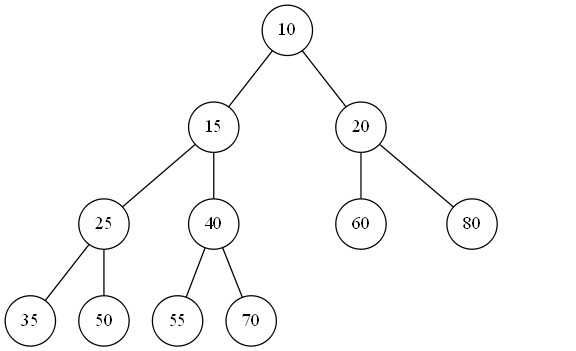
\includegraphics[scale=0.5]{minheap.png} \hspace{0.5in}
	\caption{min heap}
	\end{figure}

\paragraph{.}
The above diagram shows a min heap satisfying the two essential properties of binary heap.\newline
The essential operations on a binary heap are:\newline
\indent -INSERTION\newline
\indent -DELETION \newline
\indent\indent -Extract Min (if min heap)\newline
\indent\indent -Extract Max (if max heap)\newline 

Now we will analyse all these operation in a min heap.\newline\newline
\subparagraph{\textbf{INSERTION}\newline}
Suppose we want to insert element 5 into the min heap shown in figure 1.\newline
Steps to be followed are:\newline
\indent - Insert new node 5 into the tree maintaining complete binary tree property.\newline
\indent - Make necessary swaps to maintain heap property.\newline

\begin{figure}[h] \label{fig:png}
	\includegraphics[scale=0.4]{ins1.png} \hspace{0.5in}
	\includegraphics[scale=0.4]{ins2.png} \hspace{0.5in}
	\includegraphics[scale=0.5]{ins3.png} \hspace{0.5in}  
	\caption{Steps in Inserting 5 into min heap}	
\end{figure}

As depicted by above figure insertion of 5 causes 2 swaps and finally it becomes the new root.\newline
For a min heap after inserting the new node it is compared with its parent.If parent is greater than newnode then swap and repeat the process for parent and grand parent and so on. The process stops once we reach the root or parent becomes smaller than its child.\newline

\subparagraph{\textbf{DELETION}\newline}
Deletion in a heap always delete the root node.In case of a min-heap root is the smallest element.So deletion of root deletes the minimum that is Extract Minimum operation. In case of a max-heap root is the largest element. So deletion of root deletes the maximum element that is Extract Maximum operation.\newline\newline
Steps to be followed in delete operation are :\newline
\indent- replace the root node by the rightmost node in the bottommost level of the complete binary tree.\newline
\indent- compare the new root with its children and make necessary swapping to maintain heap property.\newline
Suppose we execute delete operation on the min heap obtained in Figure 2. The steps involved in the deletion process are shown in Figure 3.\newline\
 
\begin{figure}[h] \label{fig:png}
	\includegraphics[scale=0.5]{del1.png} \hspace{1in}
	\includegraphics[scale=0.4]{del2.png} \hspace{0.5in}
	\includegraphics[scale=0.4]{del3.png} \hspace{0.5in}  
	\caption{Steps in Delete operation in min heap}	
\end{figure}  


\section{Height of a Binary Heap\newline}

\paragraph{\textbf{Height is O(logn) :}\newline}


\begin{proof}
The height of a binary heap is the maximum number of levels from root to the leaves.\newline
Suppose the heap contains only one node that is only the root,then height is 0.If it contains 2 or 3 nodes then height is 2.\newline Root is always at level 0. So for a heap with height \textbf{h} maximum number of nodes in the last level that is maximum number of leaves can be 2\(^h\).   
If \textbf{n} is the total number of nodes and height of the heap is \textbf{h} then we have\newline\newline
\indent 2\(^0\)+2\(^1\)+2\(^2\)+- - - - - - - +2\(^h\)=n\newline
\indent 2\(^{h+1}\)=n+1\newline
\indent h+1=log(n+1)\newline
\indent h=O(logn)\newline\newline
While inserting a new node, in the worst case the node may move upto root.So insert operation is of the order of height of the heap that is O(logn).\newline
Similarly while deletion, the node replacing the root may come down to leaf level in the worst case. So again deletion is of the order of height of the heap that is O(logn).\newline  


\end{proof}

\begin{thebibliography}{}
\bibitem {}Thomas H. Cormen ,Charles E. Leiserson ,Ronald L. Rivest,Clifford Stein, \textit{Introduction to Algorithms, 3rd edition},3rd edition, 2001
\bibitem{} web resource \textit{wikipedia}
\end{thebibliography}
\end{document}
